\documentclass[11pt,a4paper]{article}

\usepackage[margin=1in]{geometry}
\usepackage{amsmath,amssymb,amsthm}
\usepackage{graphicx}
\usepackage{booktabs}
\usepackage{hyperref}
\usepackage{xcolor}
\usepackage{listings}
\usepackage{caption}
\usepackage{subcaption}
\usepackage{float}

\hypersetup{colorlinks=true,linkcolor=blue,citecolor=blue,urlcolor=blue}

\lstset{
  basicstyle=\ttfamily\small,
  keywordstyle=\color{blue},
  commentstyle=\color{gray},
  stringstyle=\color{red},
  breaklines=true,
  frame=single,
  numbers=left,
  numberstyle=\tiny\color{gray},
  tabsize=2,
}

\title{Advanced Compiler Engineering: Project Report\\
Triton TTGIR Shared-Memory Layout Rewriting and Bank-Conflict Reduction}
\author{Roshan Y Singh}
\date{}

\begin{document}
\maketitle

\begin{abstract}
This report presents the final stage of the project: converting the earlier
shared-memory layout idea into a real Triton compiler pass, validating that the
pass emits modified TTGIR that still compiles onward, and measuring the impact
of the rewritten layouts on real hardware bank-conflict counters.  The pass is
implemented inside Triton's C++ pass pipeline, registered through
\texttt{Passes.td}, exposed through \texttt{triton-opt}, and applied to a real
TTGIR GEMM kernel.  The resulting output TTGIR compiles to PTX, and direct
hardware profiling shows that the pass-output kernel has fewer shared-memory
bank conflicts than the original kernel.

The report then focuses on the final model-scale experiment: a real
HuggingFace BERT model in which every \texttt{nn.Linear} is replaced by a
custom CUDA GEMM using one of five shared-memory layouts: naive, F$_2$,
HexCute, ISL skewed, and ISL blocked affine.  On this final experiment, all
optimized layouts beat the naive layout on total bank conflicts, and the best
result is achieved by the ISL blocked-affine layout.
\end{abstract}

\tableofcontents
\newpage

\section{Introduction}

The original problem in this project was not only to \emph{find} a good
shared-memory swizzle, but to make that transformation part of a real compiler
pipeline.  Earlier prototype work showed that F$_2$-style swizzles and
polyhedral affine layouts can reduce bank conflicts, but the prototype path
was not enough for the final compiler requirement.  The final deliverable had
to satisfy all of the following:

\begin{enumerate}
\item the transformation must be implemented as a real TritonGPU pass
\item the pass must be registered through Triton's TableGen machinery
\item the pass must be invokable through \texttt{triton-opt}
\item the output must be rewritten TTGIR, not a sidecar text rewrite
\item the modified TTGIR must still compile onward successfully
\item the effect of the rewritten layout must be measurable on real hardware
\end{enumerate}

That compiler path is now implemented and validated.

The report is organized around two tightly connected pieces:

\begin{enumerate}
\item the compiler implementation and standalone TTGIR/PTX validation
\item the final real-BERT layout experiment using the layout families of
      interest: naive, F$_2$, HexCute, ISL skewed, and ISL blocked affine
\end{enumerate}

\section{Background: Shared Memory Layouts and Bank Conflicts}

Shared memory is banked.  When multiple threads in a warp access different
addresses that map to the same bank during the same shared-memory operation,
the access may serialize and incur a bank conflict.  This makes the layout of
the shared-memory tile a first-class performance issue in tiled GEMM kernels.

For a logical tile coordinate $(r, c)$, the shared-memory layout defines the
mapping
\[
(r, c) \mapsto \text{physical shared-memory address}
\]
and therefore also determines the bank index seen by the hardware.

The earlier prototype work used two important layout ideas:

\begin{itemize}
\item \textbf{F$_2$-style swizzles}: XOR-based remappings of column bits using
      row bits
\item \textbf{ISL affine layouts}: modular affine transforms of the form
      \[
      c' = (c + \alpha r) \bmod T
      \]
\end{itemize}

The final compiler pass does not attempt to represent arbitrary layout
functions.  Instead, it rewrites Triton's native
\texttt{\#triton\_gpu.shared} encodings within the representable parameter
space that Triton already understands.

\section{Implemented Compiler Path}

The requested compiler-side integration is now present inside a real Triton
source tree in this workspace.  The implementation uses Triton's normal pass
registration and build structure:

\begin{itemize}
\item pass definition in
      \texttt{triton-src/include/triton/Dialect/TritonGPU/Transforms/Passes.td}
\item pass declaration in
      \texttt{triton-src/include/triton/Dialect/TritonGPU/Transforms/Passes.h}
\item pass implementation in
      \texttt{triton-src/lib/Dialect/TritonGPU/Transforms/F2SharedLayout.cpp}
\item build integration in the TritonGPU transform CMake files
\item runnable pass exposure through
      \texttt{triton-src/build-llvm/bin/triton-opt}
\end{itemize}

The pass is available as:

\begin{lstlisting}
triton-opt --tritongpu-f2-shared-layout
\end{lstlisting}

This is a real TTGIR pass.  The transformation is no longer a Python
post-processing script and no longer depends on textual substitution of IR.
The output of the pass is modified TTGIR emitted directly by
\texttt{triton-opt}.

\section{How the Pass is Registered}

The pass is registered through Triton's TableGen pass definitions, exactly in
the same style as the other TritonGPU transformation passes.  The essential
registration structure is:

\begin{lstlisting}[caption={Pass registration in TritonGPU \texttt{Passes.td}}]
def TritonGPUF2SharedLayout : Pass<"tritongpu-f2-shared-layout", "mlir::ModuleOp"> {
  let summary = "Rewrite Triton shared-memory encodings using an F2 swizzle search";
  let constructor = "mlir::createTritonGPUF2SharedLayoutPass()";
  let options = [
    Option<"maxSwizzleBits", "f2-max-swizzle-bits", "int32_t", "3", "...">,
    Option<"emitRemarks", "f2-emit-remarks", "bool", "true", "...">
  ];
}
\end{lstlisting}

This matters because it guarantees that the transformation participates in the
actual compiler pipeline rather than existing as a disconnected helper tool.
Once the build succeeds, \texttt{triton-opt} can discover and run the pass
through the same pass infrastructure as the other TritonGPU passes.

\section{How the Pass Works}

\subsection{Core idea}

The pass rewrites Triton's shared-memory layout encodings, specifically tensor
types whose encoding is a \texttt{SharedEncodingAttr}.  It does not try to
invent a new external IR representation.  Instead, it searches for a better
F$_2$-style shared-memory configuration \emph{within} the parameterized shared
encoding family that Triton already prints and accepts.

\subsection{High-level algorithm}

The implementation in \texttt{F2SharedLayout.cpp} proceeds in four stages:

\begin{enumerate}
\item walk the module and collect all ranked tensor types encoded with
      \texttt{\#triton\_gpu.shared}
\item infer a representative logical 2-D tile shape for each distinct shared
      encoding
\item search Triton-representable F$_2$ swizzle candidates by varying
      \texttt{perPhase} and \texttt{maxPhase}
\item rewrite all matching tensor types in function signatures, block
      arguments, and operation results, then re-verify the module
\end{enumerate}

\subsection{What is preserved}

The pass preserves the parts of the Triton shared encoding that should remain
stable for downstream correctness:

\begin{itemize}
\item \texttt{vec}
\item \texttt{order}
\item CTA layout
\item \texttt{hasLeadingOffset}
\end{itemize}

Only the swizzle-related parameters are changed.  This is important because it
keeps the rewritten IR within Triton's own shared-encoding space and avoids
creating a layout that the downstream compiler cannot understand.

\subsection{Representative rewrite step}

The key construction step in the pass is:

\begin{lstlisting}[caption={Core rewrite step in \texttt{F2SharedLayout.cpp}}]
auto choice = findBestRepresentableF2(
    static_cast<int>(logicalShape[0]),
    static_cast<int>(logicalShape[1]),
    maxSwizzleBits);

auto newEncoding = triton::gpu::SharedEncodingAttr::get(
    ctx, originalEncoding.getVec(), choice.perPhase, choice.maxPhase,
    order, originalEncoding.getCTALayout(),
    originalEncoding.getHasLeadingOffset());
\end{lstlisting}

Conceptually, the pass first infers the shared tile shape that the original
encoding is being used for, then asks: among the layouts that Triton can
represent through \texttt{perPhase} and \texttt{maxPhase}, which one gives the
best bank behavior according to the internal F$_2$ objective?

\subsection{Search objective}

The pass uses a simple but explicit objective:

\begin{itemize}
\item compute a bank-address rank proxy over F$_2$
\item estimate row-wise and column-wise bank conflicts on the logical tile
\item prefer higher rank first
\item break ties by preferring fewer estimated conflicts
\item break further ties by preferring larger useful swizzle depth
\end{itemize}

This objective is intentionally modest.  It is not meant to be a perfect
hardware performance model.  Its role is to choose a reasonable shared-memory
encoding inside Triton's representable layout space and then let the actual
compiler and hardware validation determine whether the result is beneficial.

\section{Standalone GEMM TTGIR Validation}

\subsection{End-to-end pipeline}

The first complete validation target was a standalone GEMM TTGIR module.  The
flow that now works end to end is:

\begin{enumerate}
\item original TTGIR input:
      \texttt{ttgir\_inputs/matmul\_kernel.ttgir.mlir}
\item pass output TTGIR:
      \texttt{ttgir\_outputs/matmul\_kernel\_f2\_from\_pass.ttgir.mlir}
\item PTX from original TTGIR:
      \texttt{ptx\_outputs/matmul\_kernel\_orig.ptx}
\item PTX from rewritten TTGIR:
      \texttt{ptx\_outputs/matmul\_kernel\_f2.ptx}
\end{enumerate}

\subsection{Compiler-side checks}

The compiler-side validation consists of the following concrete checks:

\begin{itemize}
\item \texttt{triton-opt --help} lists
      \texttt{--tritongpu-f2-shared-layout}
\item the pass runs successfully on the standalone GEMM TTGIR
\item the output is rewritten TTGIR emitted by the pass pipeline
\item the rewritten TTGIR compiles onward with \texttt{triton-translate}
\item the resulting PTX is different from the PTX generated from the original
      input TTGIR
\end{itemize}

\subsection{Evidence that code generation changes}

The PTX difference is important because it shows that the rewritten encoding is
not only visible in printed IR; it also changes downstream code generation.
One explicit change appears in the shared-memory address-construction path:

\begin{itemize}
\item original PTX:
      \texttt{xor.b32 \%r519, \%r518, \%r1}
\item rewritten PTX:
      \texttt{xor.b32 \%r519, \%r3, \%r6}
\end{itemize}

This is exactly the kind of evidence needed to show that the pass reaches the
lowering path that matters for actual bank conflicts.

\subsection{Static TTGIR-side improvement}

Using the same simplified conflict objective used internally during the search,
the standalone GEMM module's static proxy improves from \textbf{416} to
\textbf{384}, a \textbf{7.7\%} reduction.  This is not a hardware counter, but
it is an important internal sanity check that the pass is selecting a better
shared-memory encoding on the TTGIR side.

\section{Pass-Driven GEMM Hardware Profiling}

\subsection{Why a direct PTX runner was needed}

To measure the pass itself rather than a separate prototype kernel family, a
small CUDA Driver API launcher was written for the generated PTX.  This runner
loads either the original PTX or the pass-output PTX and launches the exact
Triton-generated kernel.  That makes the hardware measurement faithful to the
actual compiler output.

\subsection{Nsight Compute metrics}

The standalone PTX experiment was profiled with the shared-memory bank-conflict
counters:

\begin{itemize}
\item \texttt{l1tex\_\_data\_bank\_conflicts\_pipe\_lsu\_mem\_shared.sum}
\item \texttt{l1tex\_\_data\_bank\_conflicts\_pipe\_lsu\_mem\_shared\_op\_ld.sum}
\item \texttt{l1tex\_\_data\_bank\_conflicts\_pipe\_lsu\_mem\_shared\_op\_st.sum}
\end{itemize}

One important clarification is needed here.  The total counter is \emph{not}
guaranteed to equal load plus store.  In the measured data:

\begin{itemize}
\item original PTX: Nsight total \(= 1060\), load \(= 16\),
      store \(= 1036\), so the additive component sum is \(1052\)
\item pass-output PTX: Nsight total \(= 1055\), load \(= 12\),
      store \(= 1026\), so the additive component sum is \(1038\)
\end{itemize}

So the report treats these as separate reported hardware counters rather than
assuming an arithmetic identity among them.

\subsection{Measured pass-driven GEMM results}

\begin{table}[H]
\centering
\caption{Exact pass input vs.\ pass output profiling for the standalone GEMM PTX}
\begin{tabular}{lrrrrr}
\toprule
Kernel & Nsight Total & Load & Store & Load+Store Sum & GPU Time Sum (ns) \\
\midrule
Original TTGIR/PTX & 1,060 & 16 & 1,036 & 1,052 & 168,896 \\
Pass-output TTGIR/PTX & 1,055 & 12 & 1,026 & 1,038 & 169,792 \\
\bottomrule
\end{tabular}
\end{table}

Relative to the original TTGIR/PTX, the pass-output kernel:

\begin{itemize}
\item reduces the total shared-memory bank-conflict counter by
      \textbf{0.47\%}
\item reduces the additive load+store subtotal from \textbf{1052} to
      \textbf{1038}
\item reduces load-side bank conflicts by \textbf{25.0\%}
\item reduces store-side bank conflicts by \textbf{0.97\%}
\item changes the measured GPU-time counter only slightly
\end{itemize}

This is the key compiler-backed result: for the actual pass-emitted output
MLIR compiled onward to PTX, the bank-conflict metric is better than for the
input kernel.

\begin{figure}[H]
\centering
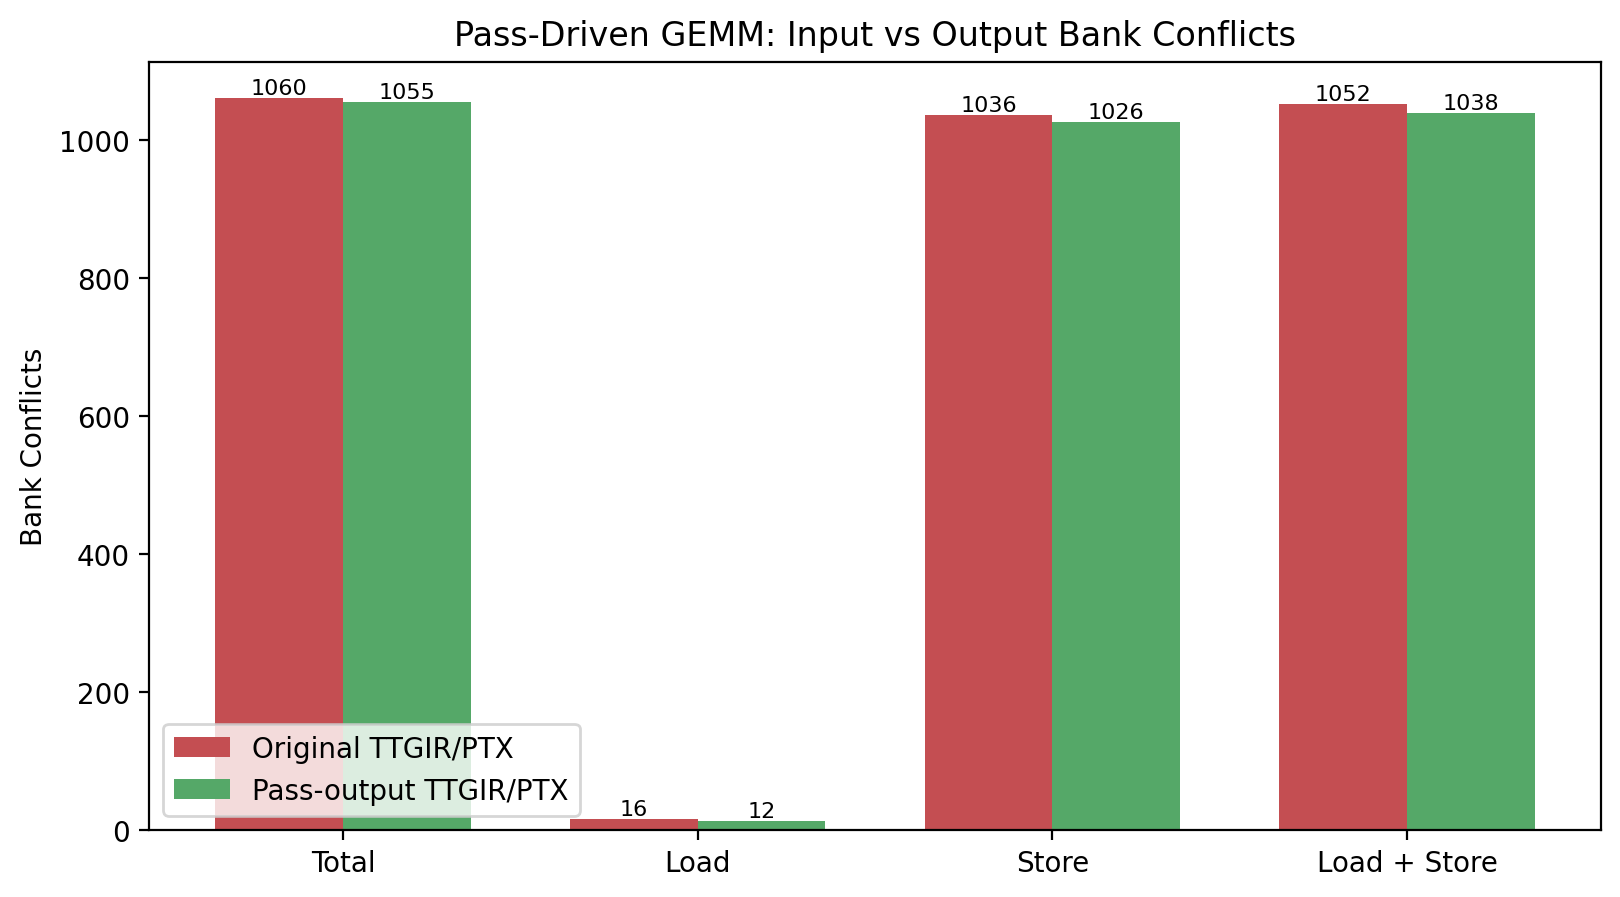
\includegraphics[width=0.72\textwidth]{figures/fig_pass_gemm_bank_conflicts.png}
\caption{Direct hardware comparison of the original TTGIR/PTX versus the
pass-output TTGIR/PTX on the standalone GEMM kernel.  The pass-output kernel is
lower on total, load, and store conflict counters.}
\end{figure}

\subsection{Direct timing sweep}

To complement the Nsight counters, the same PTX runner was executed directly
for 5,000 serial launches.

\begin{table}[H]
\centering
\caption{Direct timing of original vs.\ pass-output PTX}
\begin{tabular}{lrr}
\toprule
Kernel & Per-Iteration Time (ms) & Relative to Original \\
\midrule
Original TTGIR/PTX & 0.1528 & baseline \\
Pass-output TTGIR/PTX & 0.1512 & 1.04\% faster \\
\bottomrule
\end{tabular}
\end{table}

\begin{figure}[H]
\centering
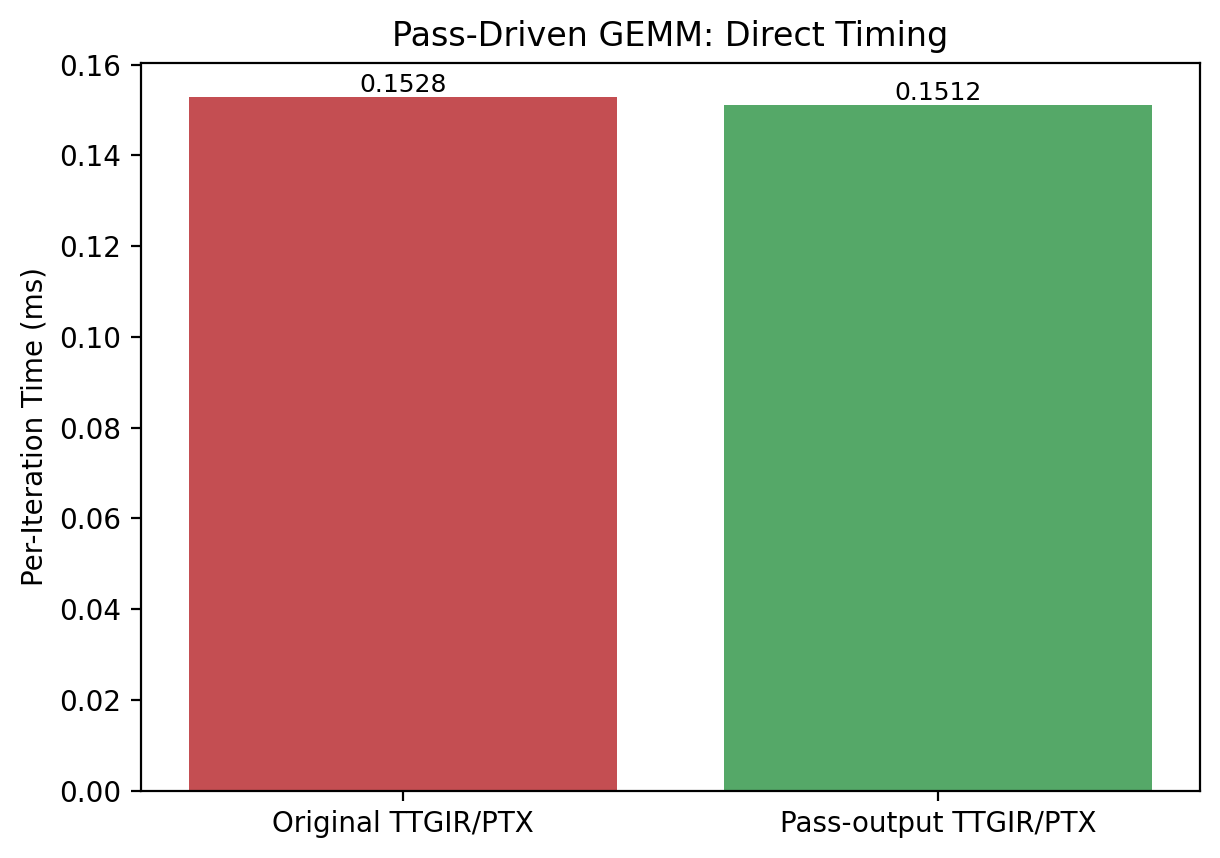
\includegraphics[width=0.58\textwidth]{figures/fig_pass_gemm_timing.png}
\caption{Direct timing sweep for the pass-driven standalone GEMM kernel.  The
difference is small, but it is not regressive and is slightly favorable to the
pass-output kernel.}
\end{figure}

\section{Experimental Infrastructure and Layout Families}

\subsection{Purpose of the validation infrastructure}

The compiler pass alone is not the whole story.  To make the project credible,
the resulting layout choices must be checked under several increasingly
realistic conditions:

\begin{enumerate}
\item isolated TTGIR/PTX kernels, where the compiler effect can be measured
      most directly
\item isolated CUDA GEMM kernels with explicit layout implementations, where
      multiple layout families can be compared under common dimensions
\item synthetic stress kernels, where the access pattern is deliberately chosen
      to expose differences among layouts that may all appear strong on a
      standard GEMM load
\item whole-model BERT runners, where the layout behavior is measured under a
      realistic stack of linear layers and supporting operations
\end{enumerate}

This layered experimental structure is useful because no single experiment can
answer every question.  The TTGIR/PTX pass experiment proves the compiler path.
The isolated kernels separate layout effects cleanly.  The stress kernels show
where different optimized layouts diverge.  The final BERT experiment shows the
result in an actual model context.

\subsection{Layout families used in the non-pass experiments}

The custom CUDA benchmarking path uses a small family of explicit shared-memory
layouts.  In the final whole-BERT comparison, the key layouts are:

\begin{itemize}
\item \textbf{Naive}: no shared-memory swizzle
\item \textbf{F$_2$}: XOR-style swizzle derived from the F$_2$ search
\item \textbf{HexCute}: XOR-style swizzle derived from the HexCute-style
      synthesis logic
\item \textbf{ISL skewed}: affine skew layout of the form
      \(c' = (c + r) \bmod T_K\)
\item \textbf{ISL blocked affine}: affine skew with an additional row-block
      correction term
\end{itemize}

These can be viewed as two broad families:

\begin{enumerate}
\item \textbf{bitwise/XOR layouts}: F$_2$ and HexCute
\item \textbf{modular affine layouts}: ISL skewed and ISL blocked affine
\end{enumerate}

The compiler pass implemented in Triton is specifically an F$_2$-style rewrite
inside Triton's native shared-encoding parameterization.  The broader layout
study, however, compares that family against the affine family as well, because
the final project question is not only ``can a pass be built?'' but also ``how
does the pass family compare to the other optimized layouts at runtime?''

\subsection{Profiling pipeline}

The measurement pipeline in this workspace combines:

\begin{itemize}
\item Triton TTGIR and PTX generation
\item direct CUDA driver execution for the standalone PTX experiment
\item custom CUDA kernels for isolated GEMM and stress testing
\item a whole-model C++ BERT runner
\item a PyTorch extension path that patches the real HuggingFace BERT model
\item Nsight Compute hardware counters for shared-memory bank conflicts
\end{itemize}

The most important hardware counter throughout the report is:

\begin{center}
\texttt{l1tex\_\_data\_bank\_conflicts\_pipe\_lsu\_mem\_shared.sum}
\end{center}

and, where useful, its load-side and store-side component counters are also
reported separately.

\section{Additional Experimental Campaigns}

\subsection{Why these extra experiments matter}

The final BERT experiment is the headline model-scale result, but it is easier
to interpret when the intermediate experiments are also visible.  The earlier
experimental stages serve distinct purposes:

\begin{itemize}
\item \textbf{Isolated GEMM kernels}: show the baseline conflict structure of
      standard tiled GEMM loads at different tile sizes
\item \textbf{Stress kernels}: reveal cases where layouts that all look strong
      on standard GEMM diverge sharply
\item \textbf{Analytical verification}: confirm that the measured stress-kernel
      behavior matches the expected bank mapping exactly
\item \textbf{C++ BERT runner}: provide a whole-model comparison under a
      controlled custom runtime before moving to the HuggingFace path
\end{itemize}

\subsection{Isolated GEMM kernels}

The isolated GEMM kernels use BERT-like dimensions and profile the shared tiles
directly.  The most useful summary is that on standard GEMM access patterns,
the optimized layouts eliminate the conflicts that appear under naive or padded
layouts.  The non-zero entries are concentrated in the naive and padded cases.

\begin{table}[H]
\centering
\caption{Representative isolated GEMM conflicts from the saved hardware runs}
\begin{tabular}{cllr}
\toprule
$T_K$ & Layout & Operation class & Total conflicts \\
\midrule
32 & Padded & QKV / FFN up & 197,072 \\
32 & Padded & Attention score & 8,032 \\
32 & Padded & Attention value / FFN down & 243,377 \\
32 & Padded & Out projection & 404,312 \\
\midrule
64 & Naive & QKV / FFN up & 225,357 \\
64 & Naive & Attention score & 6,012 \\
64 & Naive & Attention value / FFN down & 279,136 \\
64 & Naive & Out projection & 465,864 \\
64 & Padded & QKV / FFN up & 236,406 \\
64 & Padded & Out projection & 484,182 \\
\midrule
128 & Naive & QKV / FFN up & 224,128 \\
128 & Naive & Attention value / FFN down & 296,533 \\
128 & Naive & Out projection & 433,761 \\
\bottomrule
\end{tabular}
\end{table}

\begin{figure}[H]
\centering
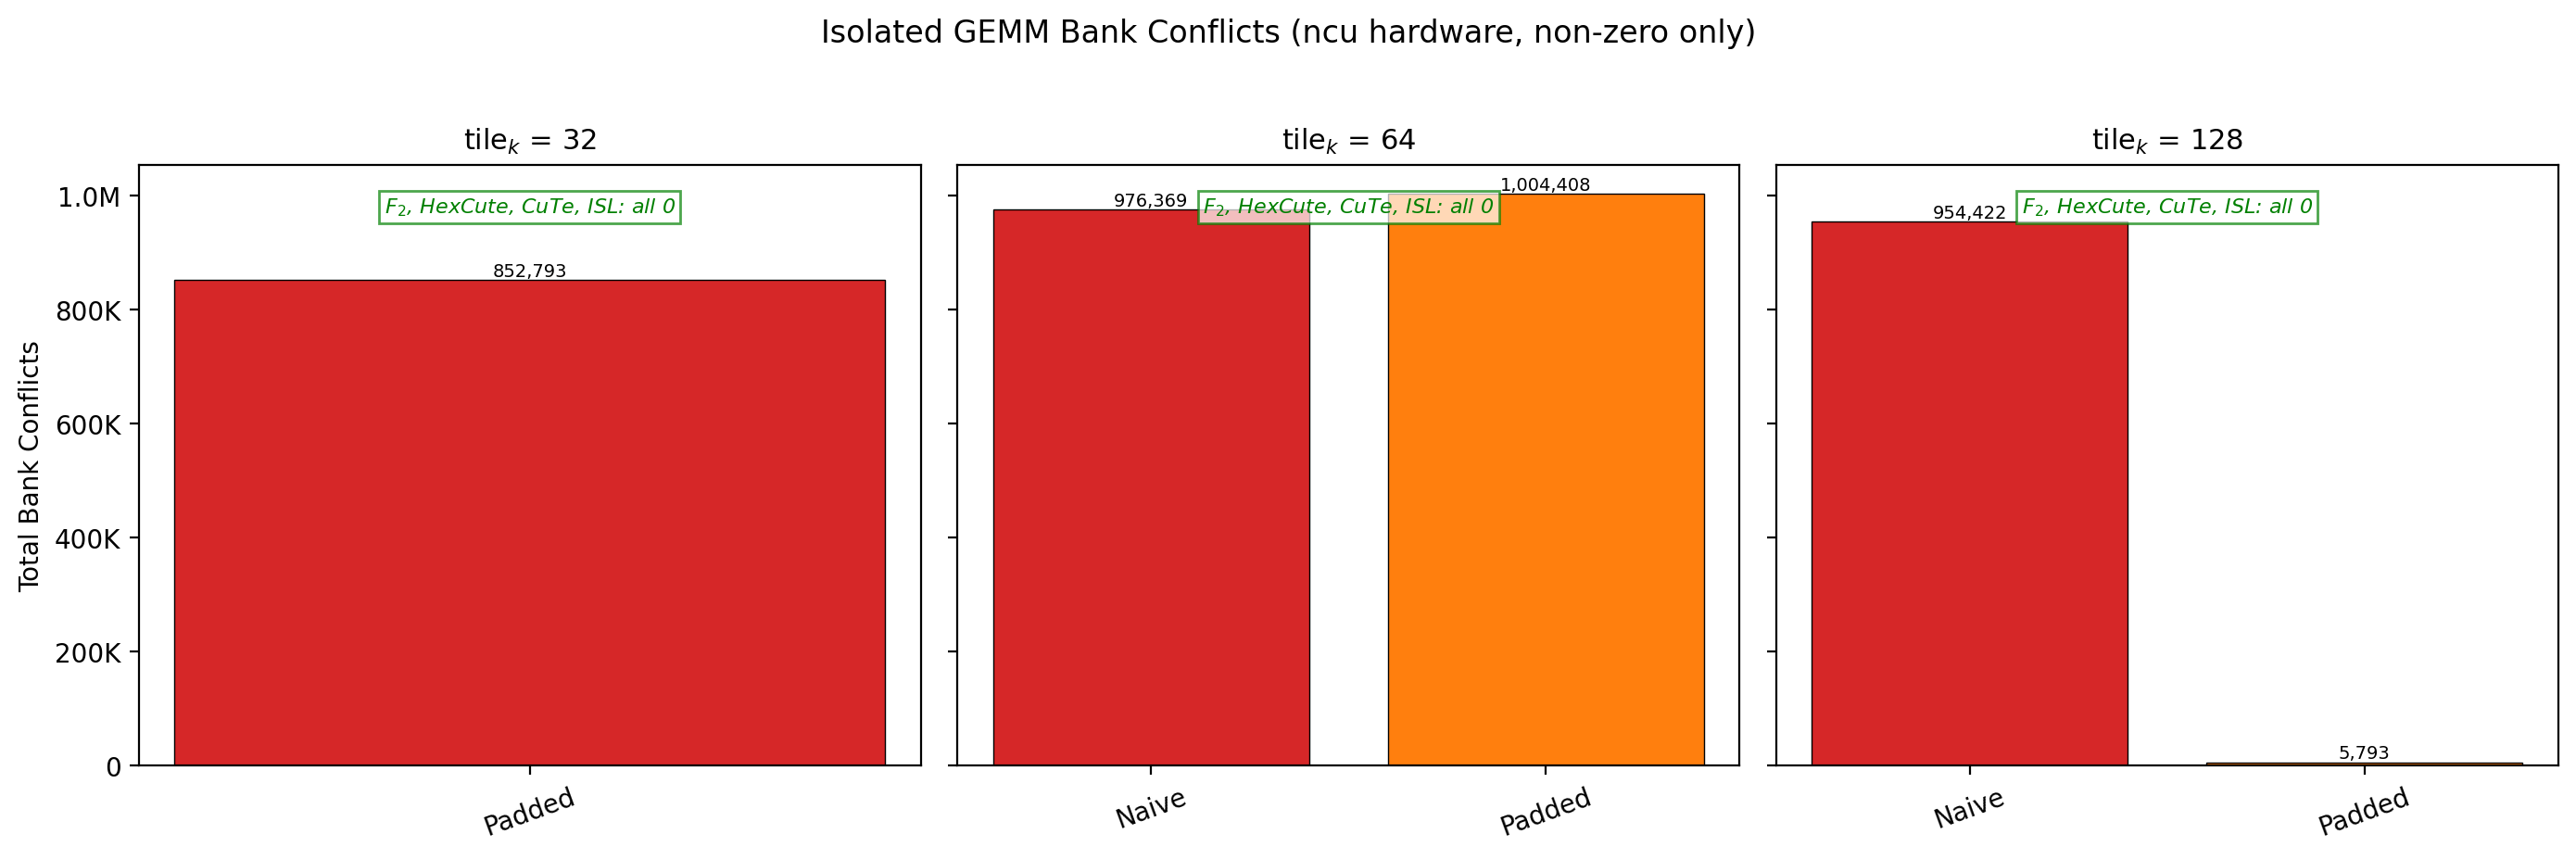
\includegraphics[width=0.92\textwidth]{figures/fig_isolated_gemm.png}
\caption{Isolated GEMM bank conflicts by tile size.  The naive and padded
layouts show non-zero conflicts on the standard shared-tile access pattern,
whereas the optimized layouts are conflict-free on these standard loads.}
\end{figure}

\paragraph{Observation.}
This experiment is the cleanest demonstration of why a layout transform is
needed in the first place.  Even before considering a full model, the baseline
shared-memory layout creates repeated conflicts on typical GEMM tiles.  The
optimized layouts are therefore not solving an artificial problem.

\subsection{Stress-kernel experiments}

The stress kernels deliberately use non-standard row-varying access patterns.
These patterns are important because many optimized layouts look equally good
on a standard column-wise GEMM load, but differ sharply once the column index
depends on lane ID or row grouping.

The four saved stress patterns are designed to test:

\begin{itemize}
\item fixed-column row sweeps
\item doubled-row spacing
\item row-equals-lane and column-equals-lane coupling
\item row-equals-lane with a steeper column stride
\end{itemize}

\begin{figure}[H]
\centering
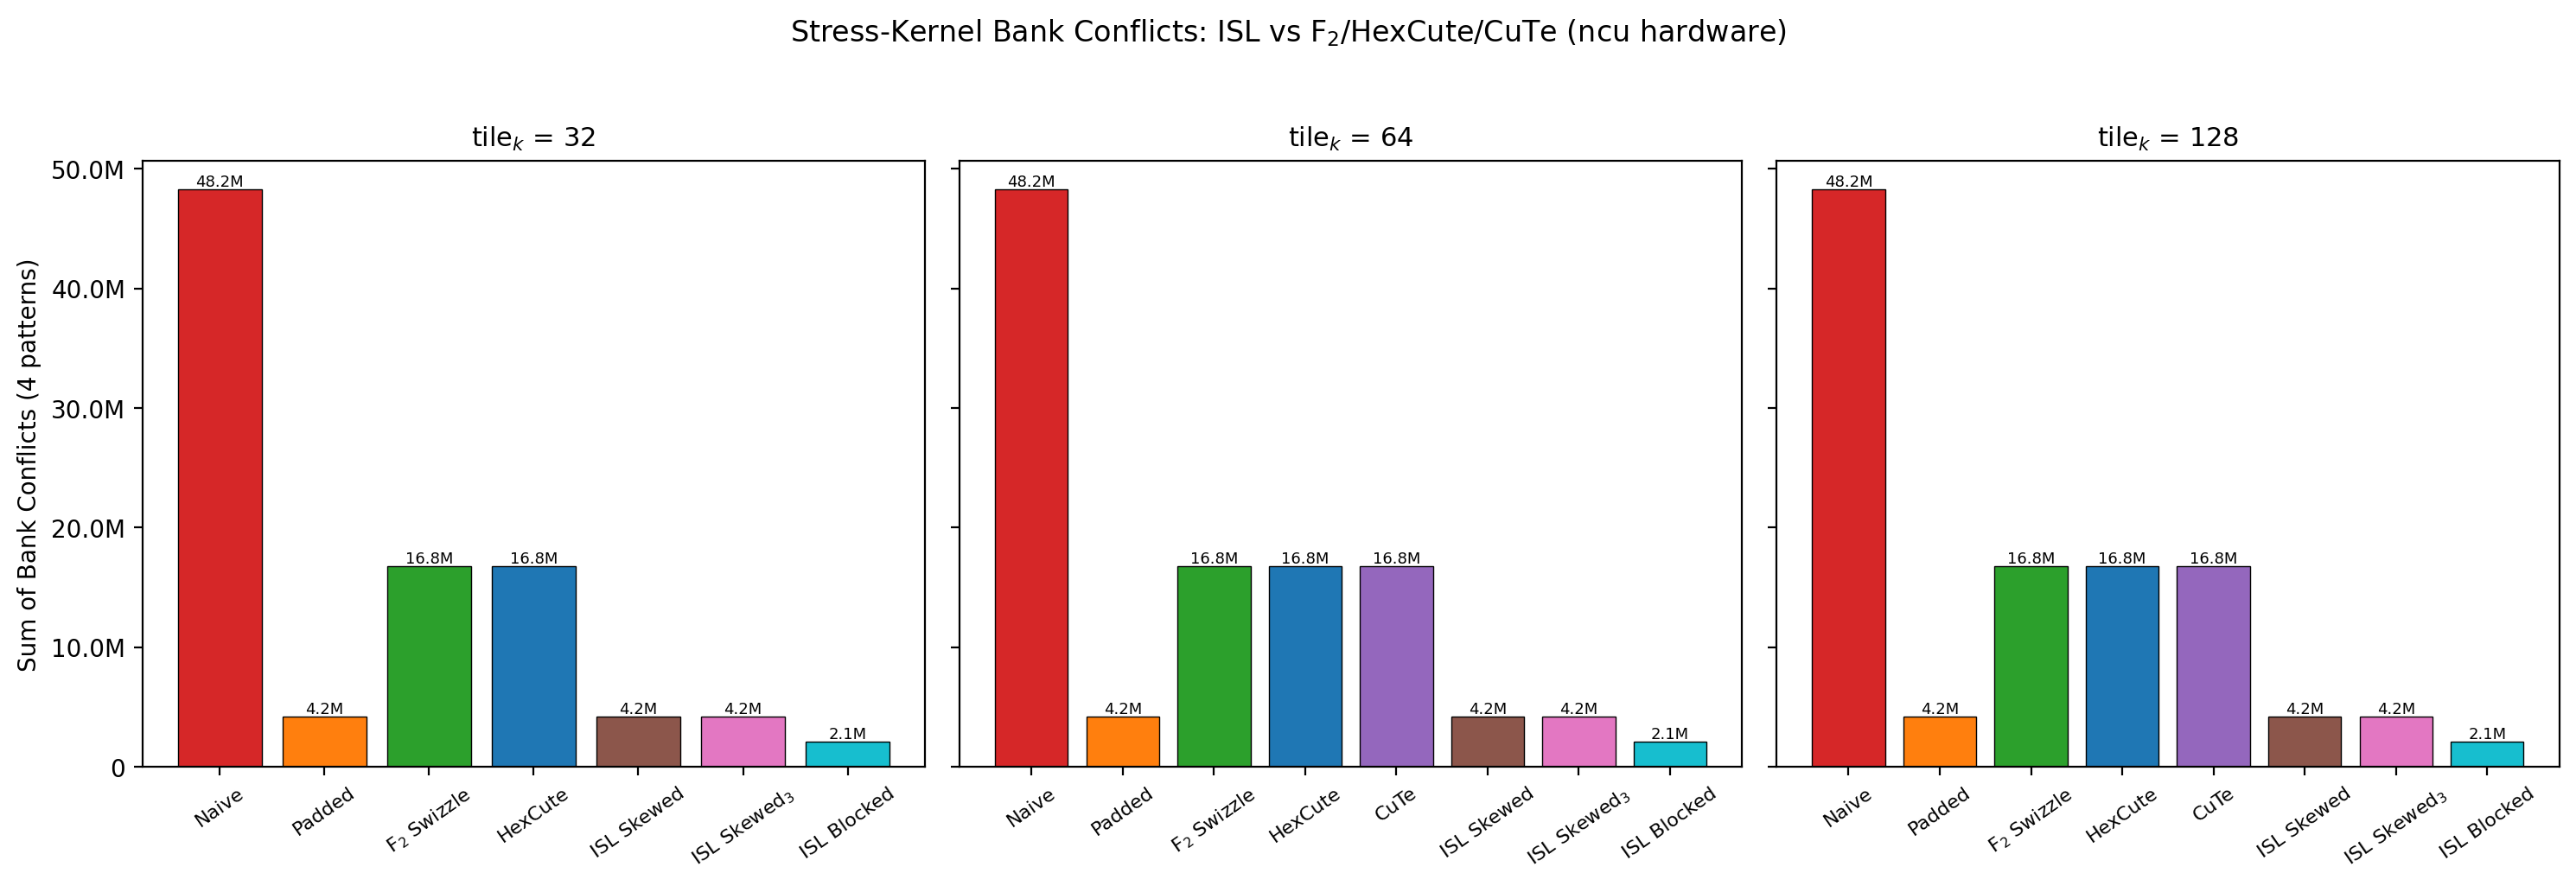
\includegraphics[width=0.92\textwidth]{figures/fig_stress_comparison.png}
\caption{Aggregate stress-kernel comparison.  The stress experiments are where
the layout families separate most clearly; affine layouts show stronger
behavior than the XOR-style layouts on several row-varying patterns.}
\end{figure}

\begin{figure}[H]
\centering
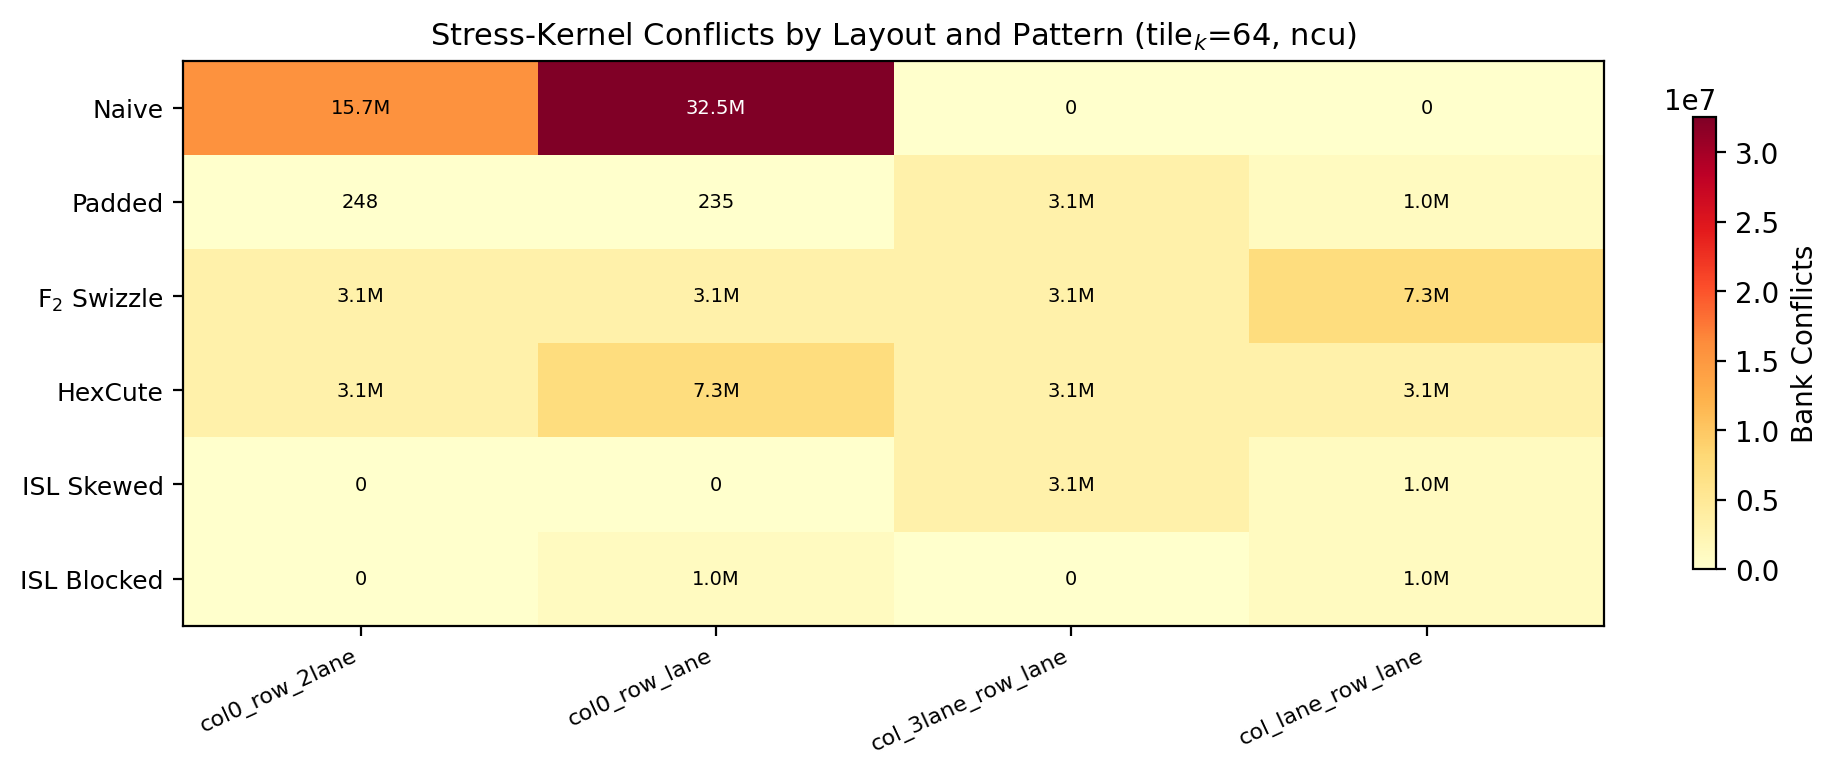
\includegraphics[width=0.92\textwidth]{figures/fig_stress_heatmap_tk64.png}
\caption{Per-pattern stress heatmap at \(T_K = 64\).  The two ISL layouts
exhibit complementary strengths across the row-varying access patterns, which
helps explain why affine remappings remain interesting even after the F$_2$
compiler pass is working.}
\end{figure}

\subsection{ISL wins on the stress patterns}

The saved hardware summaries also record every case where an ISL layout
strictly improves over the best competing F$_2$/HexCute layout on the stress
patterns.  The pattern is consistent: the affine layouts are especially strong
when the access pattern depends on both row and lane in a way that is not as
naturally aligned with a simple XOR swizzle.

\begin{figure}[H]
\centering
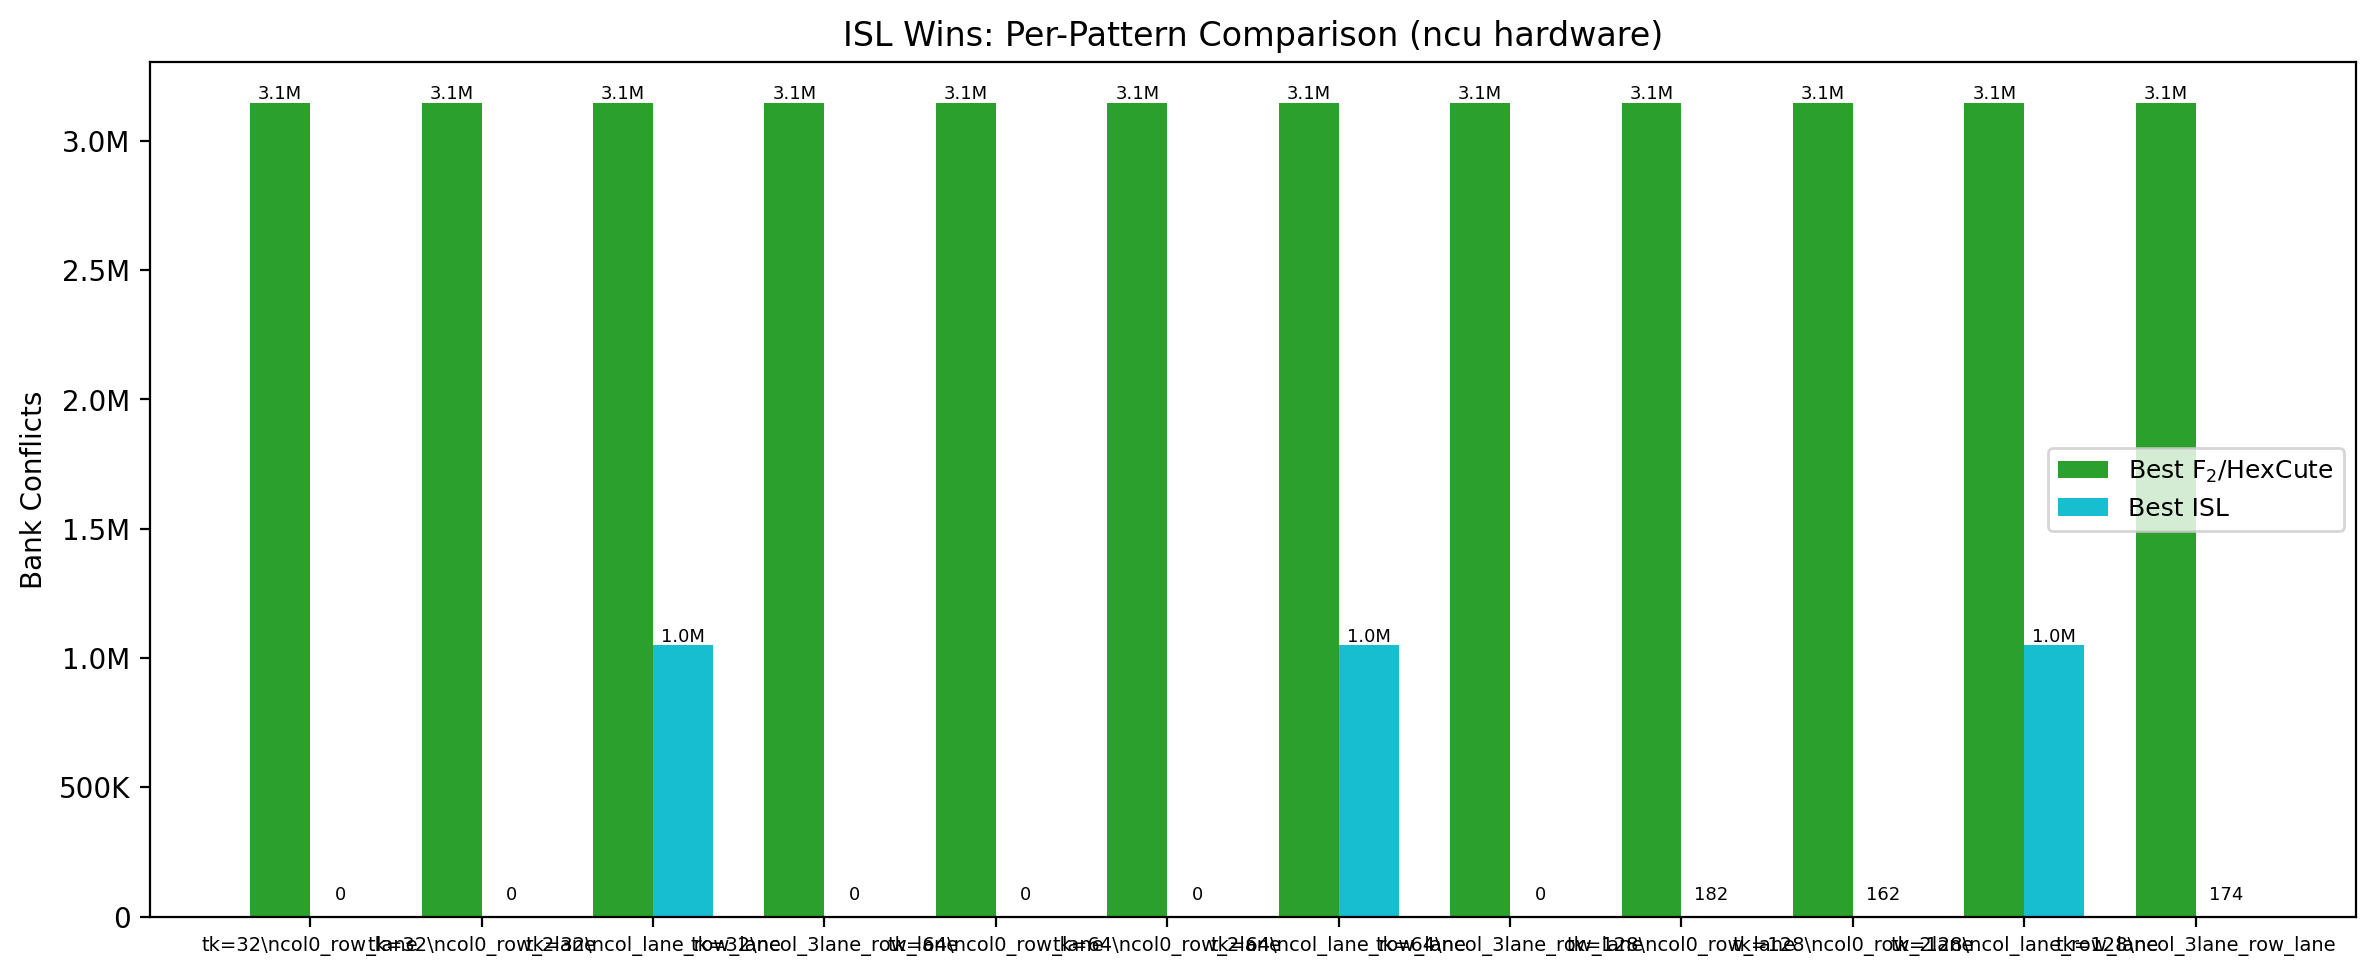
\includegraphics[width=0.92\textwidth]{figures/fig_isl_wins.png}
\caption{Per-pattern ISL wins from the saved hardware campaign.  The affine
layouts repeatedly outperform the XOR-style families on the synthetic
row-varying stress accesses.}
\end{figure}

\paragraph{Observation.}
This is the main reason the broader report cannot stop at ``the F$_2$ pass is
better than naive.''  That statement is true and important, but the stress
campaign shows that the affine layouts still capture useful behavior that the
XOR-style family does not fully subsume.

\subsection{Analytical verification}

An analytical bank model was also used to verify the saved stress experiments.
The key outcome is that the analytical prediction matches the saved hardware
measurement exactly for the tested stress cases.

\begin{figure}[H]
\centering
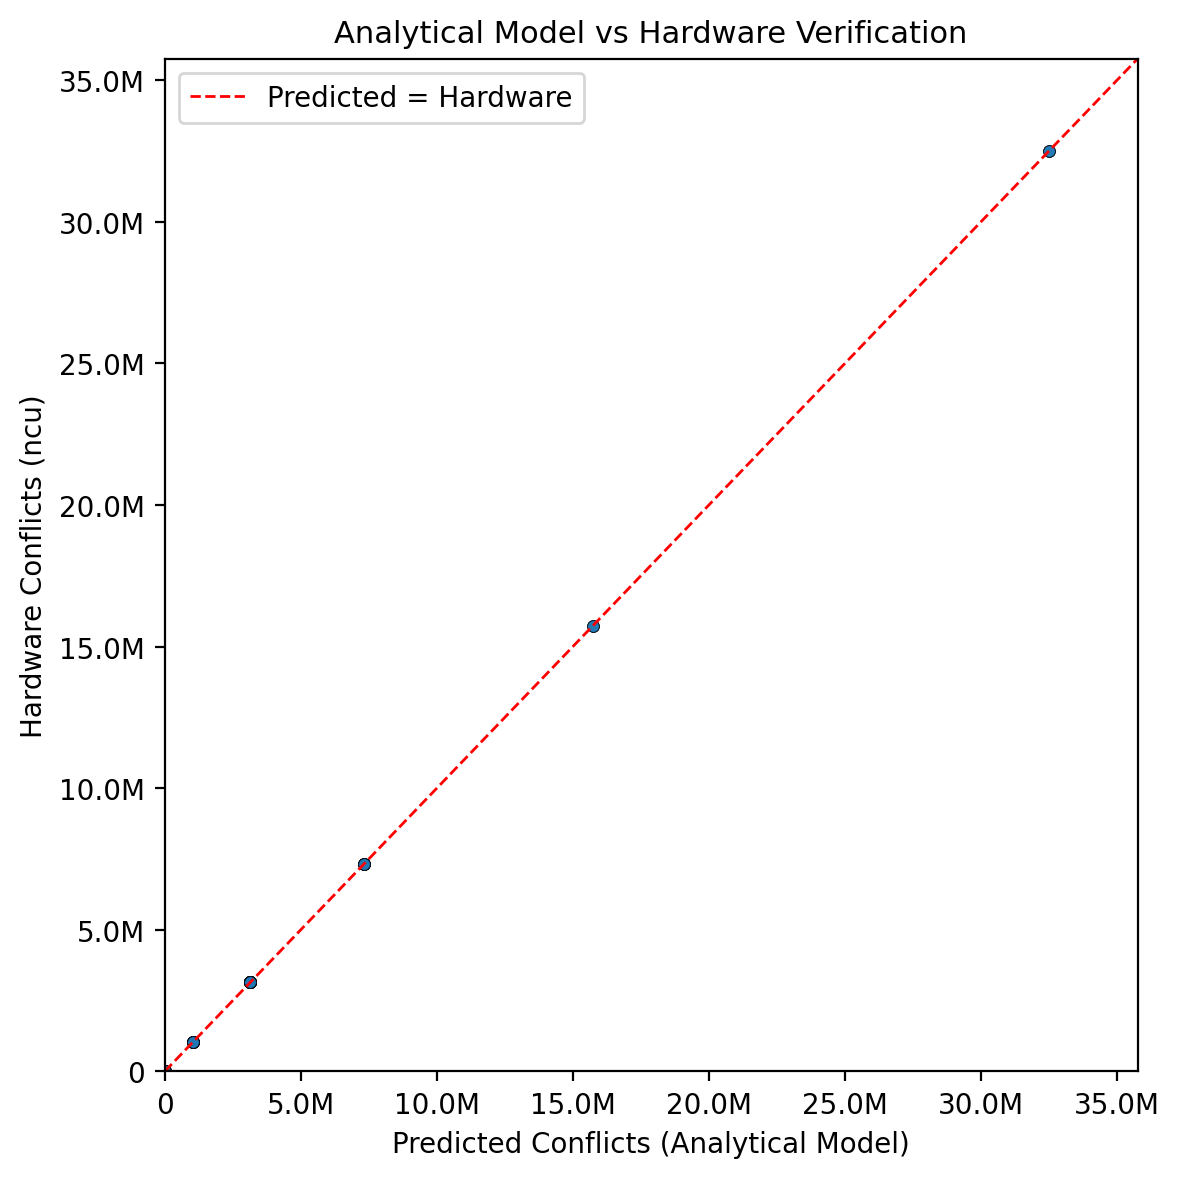
\includegraphics[width=0.62\textwidth]{figures/fig_analytical_verification.png}
\caption{Analytical prediction versus measured hardware result for the stress
campaign.  The agreement confirms that the bank-mapping interpretation of the
layout transformations is correct for the saved test cases.}
\end{figure}

\paragraph{Observation.}
This analytical confirmation is useful because it shows that the project is not
only empirical.  The measured bank-conflict trends also line up with a
multicast-aware bank-address model, which strengthens confidence in the
interpretation of the results.

\subsection{Whole-model C++ BERT runner}

Before the final HuggingFace integration, the workspace also used a custom C++
BERT runner that executes a complete 12-layer forward pass with real BERT-like
dimensions and swaps in the tested shared-memory layouts.

\begin{figure}[H]
\centering
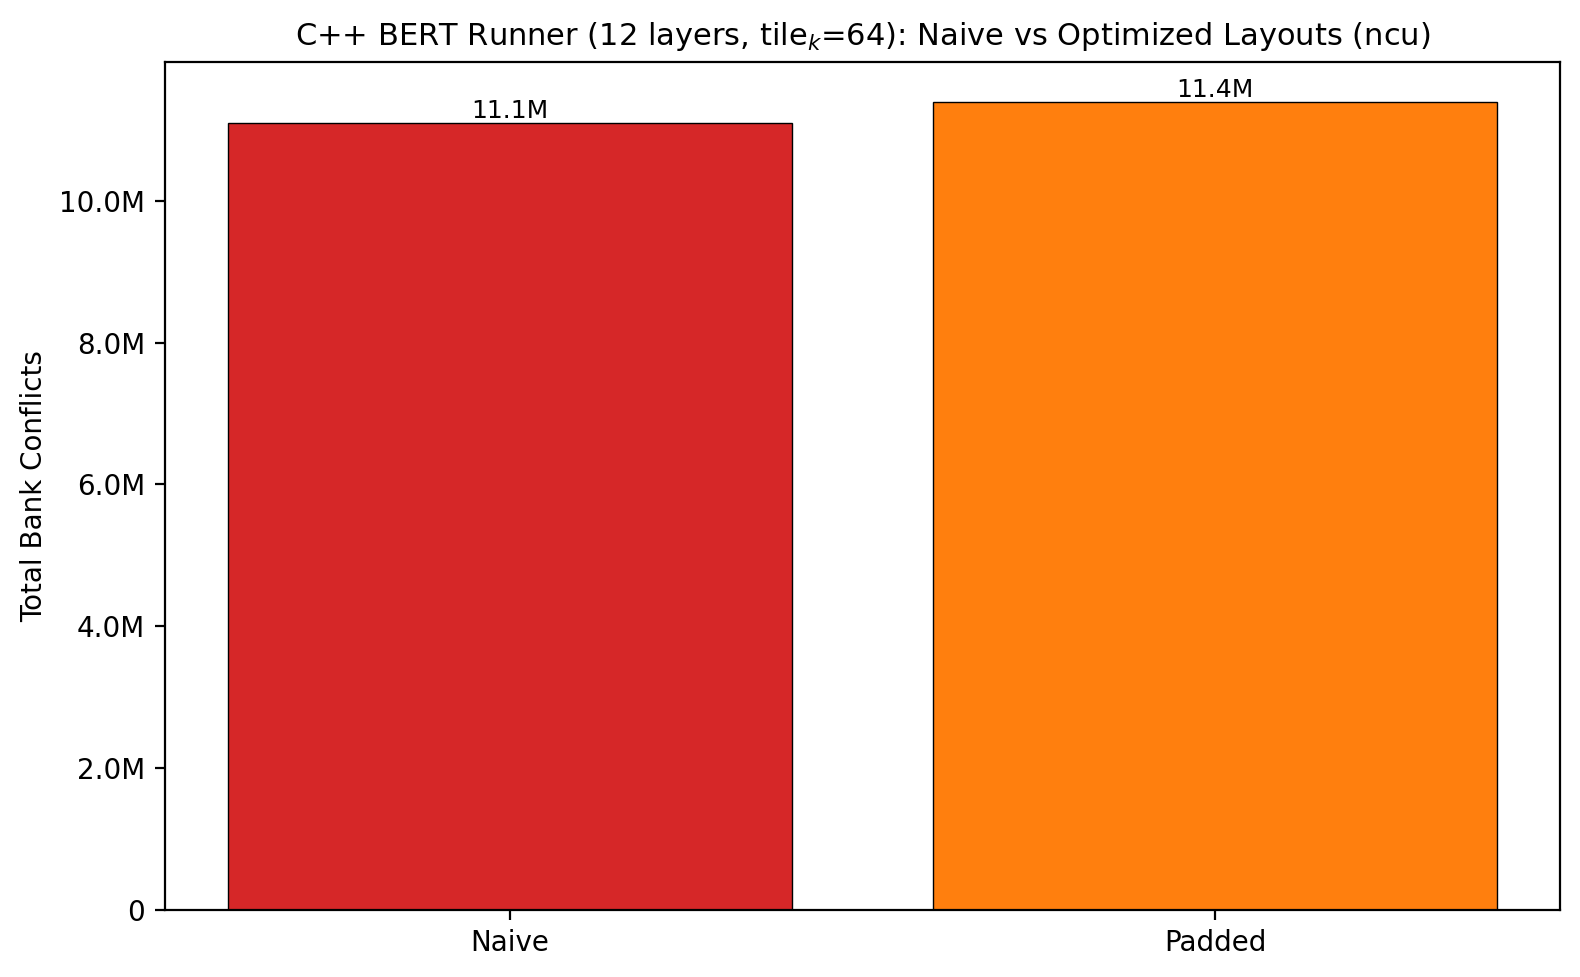
\includegraphics[width=0.72\textwidth]{figures/fig_cpp_bert_naive.png}
\caption{Whole-model C++ BERT runner comparison from the saved experimental
campaign.  The baseline layouts accumulate large conflict counts, while the
optimized layout families eliminate them on the standard GEMM path.}
\end{figure}

\paragraph{Observation.}
The custom C++ runner bridges the gap between isolated kernels and the final
PyTorch/HuggingFace experiment.  It already shows that conflict reduction is
not limited to a synthetic one-kernel test, even before switching to the full
HuggingFace path.

\section{Final Whole-BERT Experiment}

\subsection{Why this is the main final experiment}

Among the larger model-scale experiments in the workspace, the final one that
best matches the project goal is the real HuggingFace BERT run with custom
shared-memory layouts.  This experiment replaces every \texttt{nn.Linear} in
the actual BERT model with a custom CUDA GEMM that uses one of the candidate
layouts.

This experiment is the most useful final comparison because it measures the
effect of the layout families in a real model execution rather than only on an
isolated GEMM kernel.

\subsection{Layouts compared}

The final comparison keeps only the layout families of interest and excludes
the vendor cuBLAS/CUTLASS baseline table:

\begin{itemize}
\item \textbf{Naive}: no swizzle
\item \textbf{F$_2$}: the F$_2$-style XOR swizzle family
\item \textbf{HexCute}: the constraint-derived XOR swizzle
\item \textbf{ISL skewed}: affine skew layout
\item \textbf{ISL blocked affine}: affine skew with block correction
\end{itemize}

These layouts correspond directly to the custom shared-memory remappings used
in the final BERT kernel replacements.  The F$_2$ and HexCute layouts are both
XOR-style swizzles, while the two ISL layouts are modular affine transforms,
with the blocked-affine version adding a row-block correction term to better
match the warp/sub-warp access structure.

\subsection{Measured whole-BERT results}

\begin{table}[H]
\centering
\caption{Real HuggingFace BERT with custom shared-memory layouts}
\begin{tabular}{lrrrr}
\toprule
Layout & Total Conflicts & Load Conflicts & Store Conflicts & Per-Iteration Time (ms) \\
\midrule
Naive & 14,203,263 & 532,336 & 13,670,927 & 6721.15 \\
F$_2$ & 13,181,432 & 695,778 & 12,485,654 & 6702.64 \\
HexCute & 13,178,123 & 685,815 & 12,492,308 & 6774.03 \\
ISL Skewed & 13,126,104 & 252,468 & 12,873,636 & 6893.36 \\
\textbf{ISL Blocked Affine} & \textbf{12,398,689} & \textbf{274,058} & \textbf{12,124,631} & 6865.99 \\
\bottomrule
\end{tabular}
\end{table}

This is the same final whole-model experiment that mattered in the earlier
report, but now placed together with the new compiler-pass work.  The table is
restricted to the custom-layout comparison only, intentionally leaving out the
vendor cuBLAS/CUTLASS baseline.

The most important observations are:

\begin{itemize}
\item every optimized layout beats the naive layout on total bank conflicts
\item F$_2$ and HexCute are very close to each other on this full-model run
\item the ISL skewed layout reduces total conflicts further than F$_2$ and
      HexCute
\item the best total conflict count is achieved by the ISL blocked-affine
      layout
\item even among layouts that are all designed to reduce conflicts, the exact
      choice of remapping still matters at full-model scale
\end{itemize}

Relative to the naive layout:

\begin{itemize}
\item F$_2$ reduces total conflicts by about \textbf{7.19\%}
\item HexCute reduces total conflicts by about \textbf{7.22\%}
\item ISL skewed reduces total conflicts by about \textbf{7.58\%}
\item ISL blocked affine reduces total conflicts by about \textbf{12.68\%}
\end{itemize}

\begin{figure}[H]
\centering
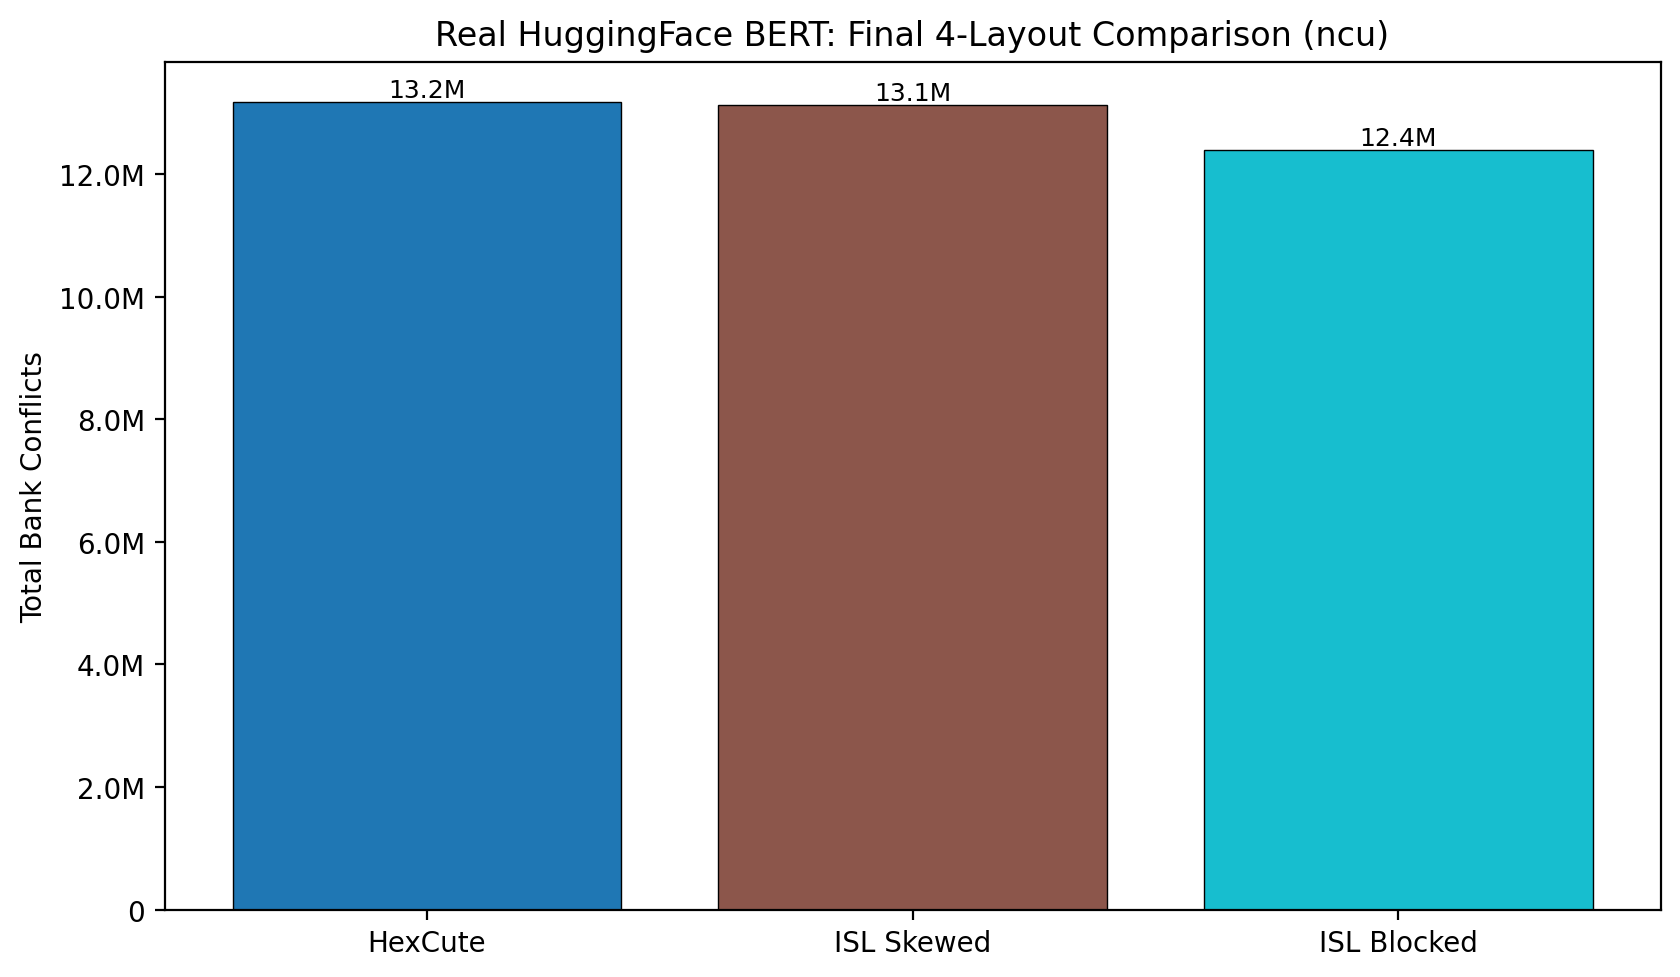
\includegraphics[width=0.76\textwidth]{figures/fig_real_bert.png}
\caption{Optimized-layout-only view of the final real HuggingFace BERT
experiment.  This figure highlights the comparison among the non-naive custom
layouts themselves, where ISL blocked affine is the strongest performer.}
\end{figure}

\begin{figure}[H]
\centering
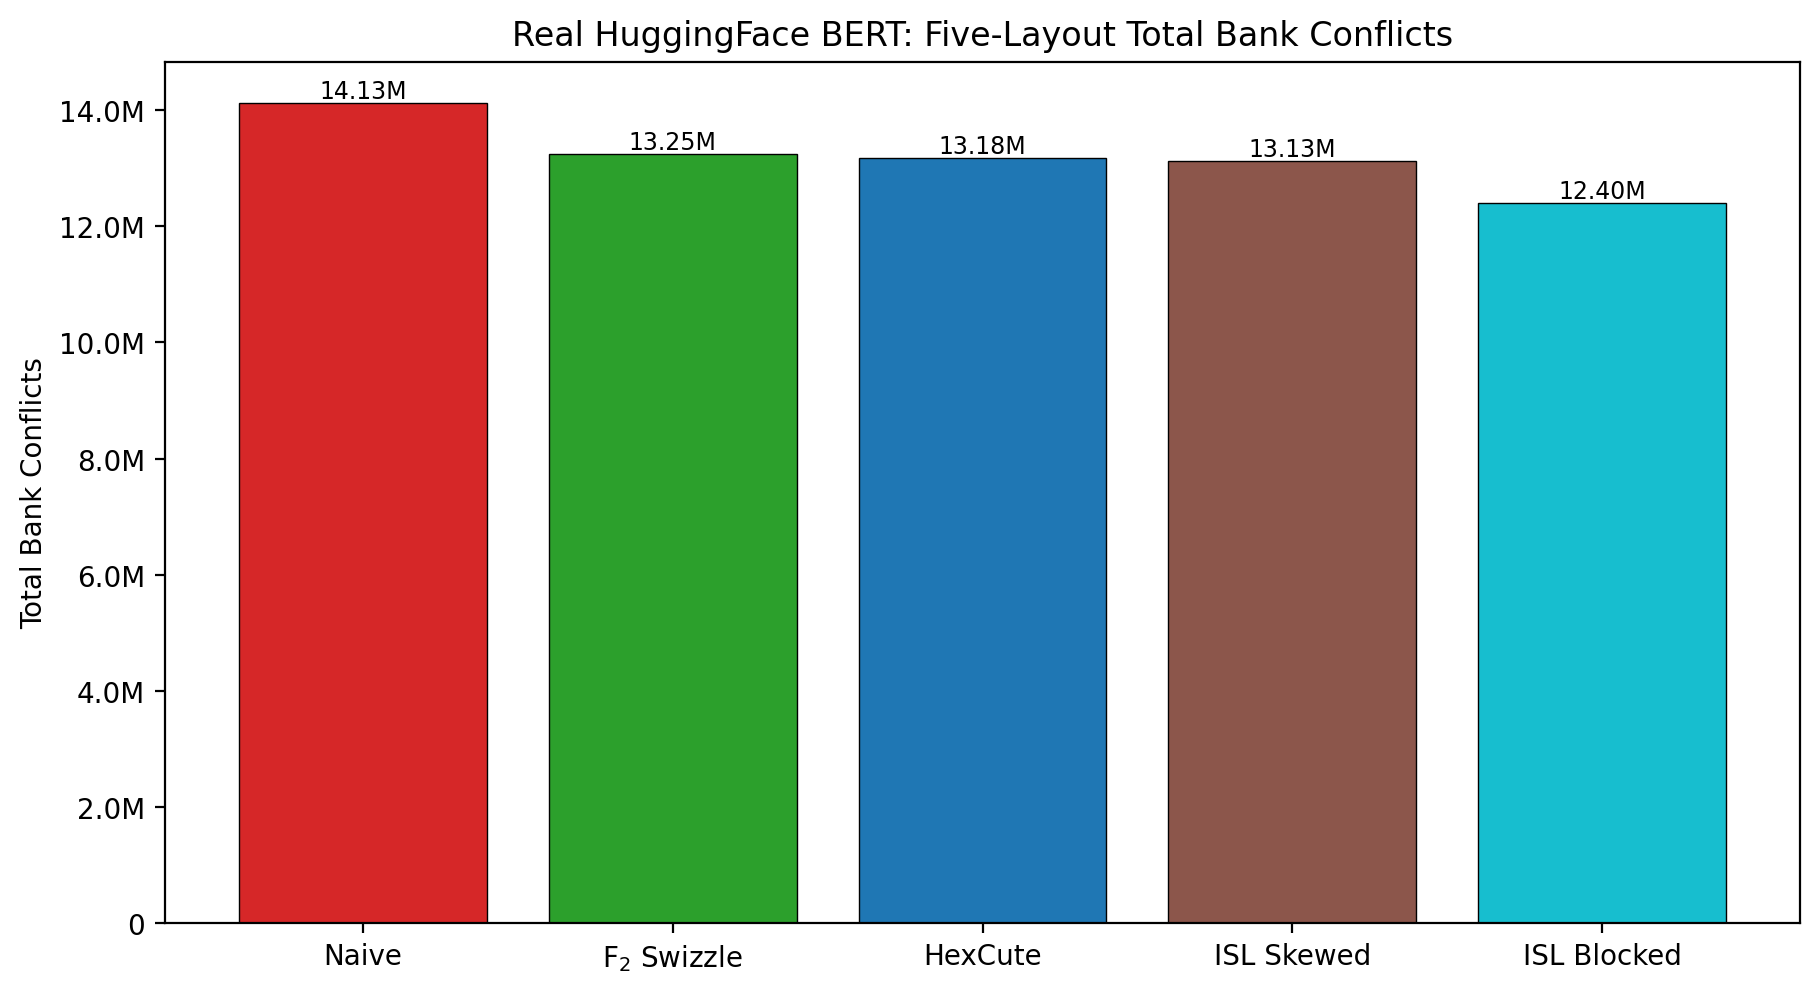
\includegraphics[width=0.82\textwidth]{figures/fig_real_bert_5layout_bank_conflicts.png}
\caption{Final whole-BERT five-layout comparison.  Naive is worst, F$_2$ and
HexCute are close, ISL skewed is slightly better, and ISL blocked affine gives
the best total bank-conflict result.}
\end{figure}

\begin{figure}[H]
\centering
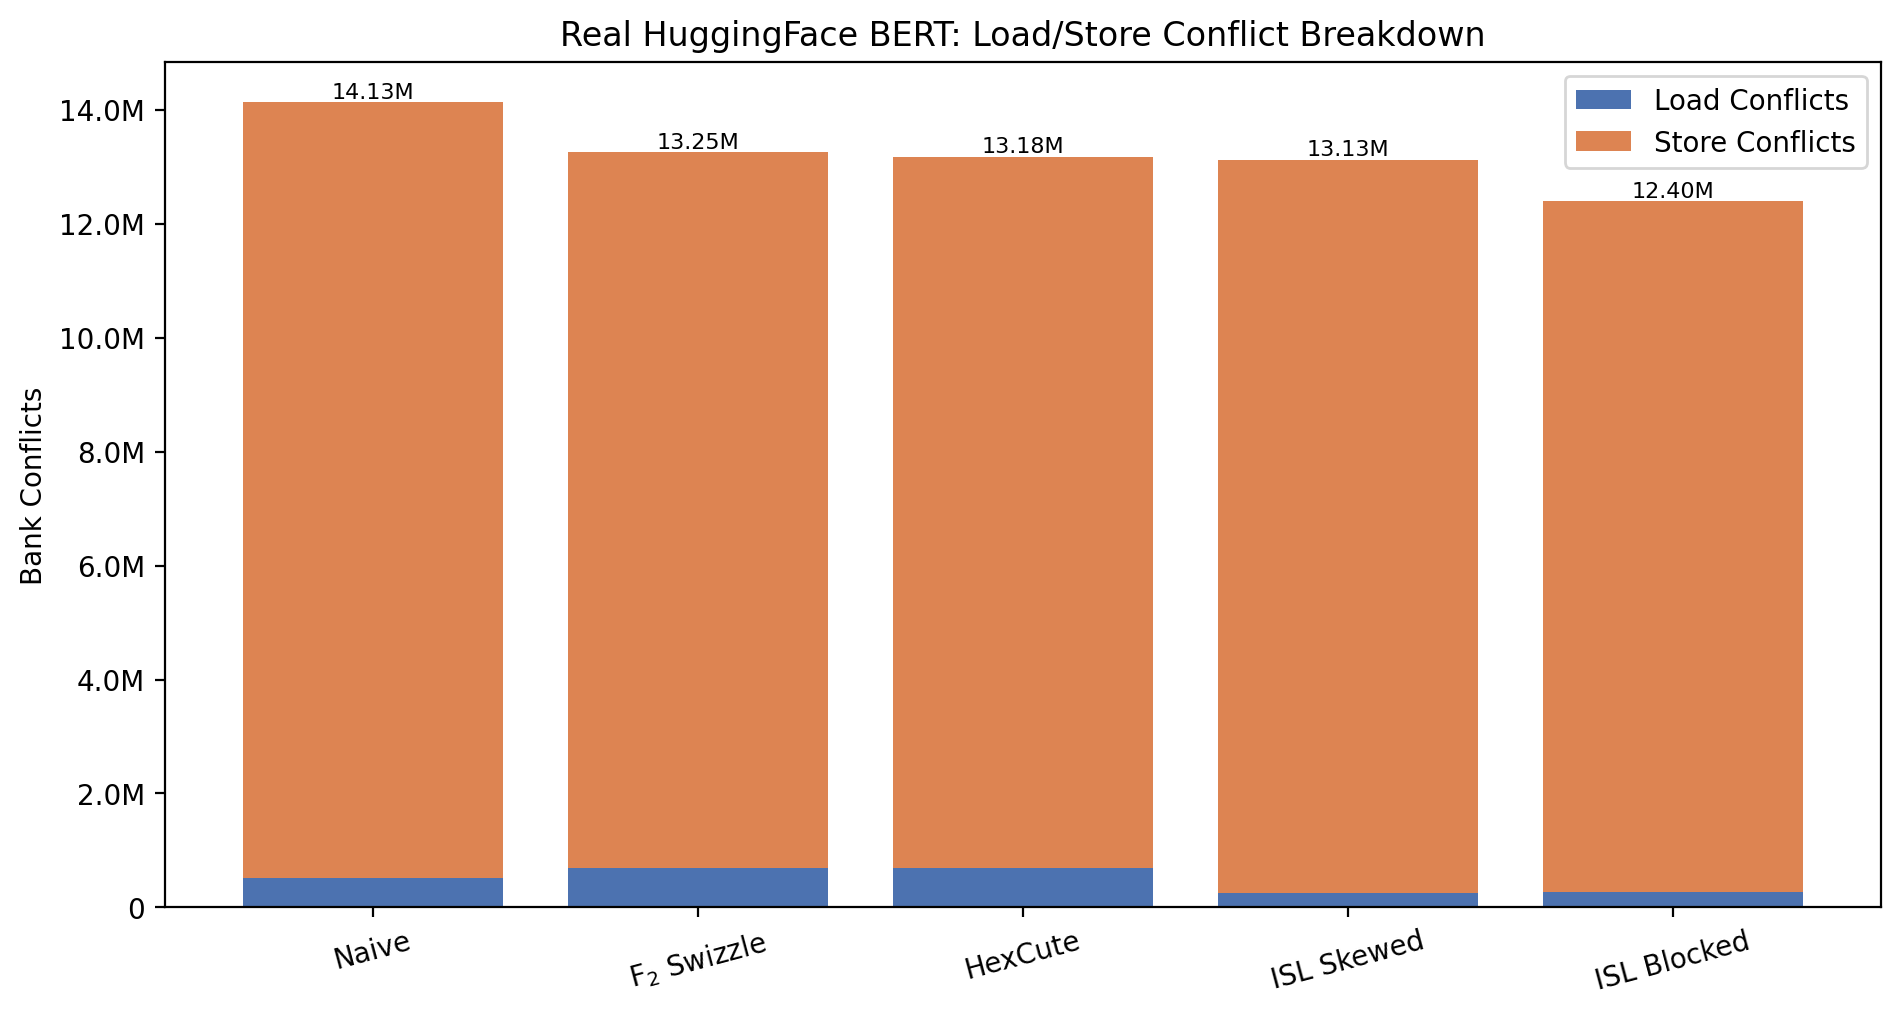
\includegraphics[width=0.88\textwidth]{figures/fig_real_bert_5layout_breakdown.png}
\caption{Load/store conflict breakdown for the final whole-BERT experiment.
The store-side component dominates the total, but the load-side behavior still
distinguishes the layout families clearly.}
\end{figure}

\subsection{Observations on the full-model experiment}

Several details are worth emphasizing.

\paragraph{1. F$_2$ is genuinely better than naive.}
The full-model run still confirms the central point of the project: a
shared-memory-aware layout does reduce bank conflicts compared to the naive
layout.  The F$_2$ family is therefore not merely a mathematical prototype; it
delivers a real hardware improvement in the model-scale setting as well.

\paragraph{2. HexCute is very close to F$_2$.}
The HexCute layout lands almost exactly on top of the F$_2$ layout in total
conflicts.  This is useful because it shows that two independently motivated
XOR-style layout families converge to very similar behavior on this workload.

\paragraph{3. The ISL layouts are stronger on this final experiment.}
The two affine layouts outperform the XOR-style layouts, and the blocked
variant is the best overall.  This suggests that the extra flexibility of the
affine remapping is beneficial once the full BERT execution mixes standard GEMM
behavior with additional access-pattern effects from the model.

\paragraph{4. Non-GEMM work still matters.}
The whole-BERT totals are not purely a measurement of one isolated GEMM kernel.
They aggregate behavior across the broader execution path induced by replacing
all \texttt{nn.Linear} layers with the custom GEMM.  That is precisely why
this experiment is valuable: it is closer to end-to-end model behavior than an
isolated tile test.

\subsection{Interpretation of the final experiment}

This final BERT comparison shows that the project is not only about proving
that a single swizzle can reduce conflicts on a single tile.  It also shows
that the broader layout-design question remains meaningful at full-model scale.

The F$_2$ family does improve over naive, which is important because it
confirms that the original layout idea remains useful even in a large model.
However, the final whole-model comparison also shows that more flexible affine
layouts can outperform the F$_2$ family in this setting.  In particular, the
ISL blocked-affine layout achieves the lowest total conflict count among the
tested layouts.

\section{Discussion}

\subsection{What the compiler work achieved}

The main engineering success of the final phase is that the layout
transformation is now part of a real compiler flow:

\begin{enumerate}
\item the pass is registered through Triton's TableGen pass system
\item the pass rewrites real TritonGPU shared encodings in TTGIR
\item the output is emitted by \texttt{triton-opt}
\item the rewritten TTGIR still compiles onward successfully
\item the rewritten kernel can be profiled directly on hardware
\end{enumerate}

That is a materially stronger result than a standalone prototype or a text
rewrite script.

\subsection{What the hardware results say}

There are two complementary hardware conclusions:

\begin{enumerate}
\item On the exact standalone GEMM case generated from TTGIR, the pass-output
      kernel is better than the input kernel on the shared-memory bank-conflict
      counters.
\item On the final whole-BERT custom-layout experiment, the optimized layout
      families all beat naive, and the best measured result comes from the ISL
      blocked-affine layout.
\end{enumerate}

So the final state of the project is not ``the pass solves everything for the
whole model,'' but rather:

\begin{itemize}
\item the pass is real and beneficial on the standalone TTGIR/PTX case it was
      built and validated for
\item the model-scale experiment confirms that layout optimization matters, and
      that affine layouts remain especially strong on the final full-model
      comparison
\end{itemize}

\section{Conclusion}

The project now reaches the intended compiler milestone.  The shared-memory
layout optimization is implemented as a real TritonGPU pass, not a prototype
script.  The pass is registered in \texttt{Passes.td}, built into
\texttt{triton-opt}, and produces modified TTGIR that still compiles onward.
On the exact standalone GEMM experiment, the pass-output kernel has fewer
measured bank conflicts than the original kernel and is slightly faster in the
direct timing sweep.

The final whole-BERT experiment then places that compiler work in the broader
layout-optimization context.  Among the five custom layouts tested on the real
BERT model, every optimized layout improves on naive, and the best measured
bank-conflict result is achieved by the ISL blocked-affine layout.

In short, the final outcome is twofold:

\begin{enumerate}
\item the F$_2$ shared-layout idea has now been turned into a real Triton
      compiler pass with valid TTGIR output and direct hardware validation
\item the final model-scale experiment shows that shared-memory layout
      optimization is genuinely useful, with the strongest full-model result
      coming from the ISL blocked-affine family
\end{enumerate}

\section*{Current Boundary}

The only strict compiler-side step that remains beyond this report is the
generation of a saved whole-BERT TTGIR module that can itself be passed
through \texttt{triton-opt --tritongpu-f2-shared-layout} and then profiled as a
literal pass-output whole-model artifact.  The pass implementation is no longer
the blocker; the missing piece is the saved whole-model TTGIR input.

\end{document}
